\documentclass{style/CRPITStyle}
\usepackage{epsfig}   % Packages to use if you wish
\usepackage{lscape}   %
\usepackage[authoryear]{natbib}
\renewcommand{\cite}{\citep}
\pagestyle{empty}
\thispagestyle{empty}
\hyphenation{roddick}

\begin{document}

\title{Software Development: An Evaluation of KPSmart Development}
\author{David Barnett}
\affiliation{School of Engineering and Computer Science \\
Victoria University of Wellington, \\
PO Box 600, Wellington, 6140 \\
Email:~{\tt barentdavi@myvuw.ac.nz}}

\maketitle

\begin{abstract}
\end{abstract}

\vspace{.1in}

\noindent {\em Keywords:}\/ System, Iterative and Incremental Development, Group Project

\vspace{.1in}

\section{Introduction}

% Which process model your team has chosen for the project and why, and
% how your team used the process model,
\section{Process Model}
% chose Spiral, moved to Incremental and Iterative (not enough risk)
% used it so we could be flexible with iteration times
% no goals for each iteration
% ending up being every iteration just being a client meeting

For the KPSmart application our team chose the to use the spiral model for our
process model. We chose this model because of its iterative approach to the
development of the application so we could get as much client feedback as we
could. We also saw risks involving our scheduling of the team to meet up and other aspects
of our project so the spiral model fitted the bill. An illustration of how the
spiral model is generically use shown in figure \ref{spiral-model}.

\vspace{.1in}

\begin{figure}[htb]
\fbox{\parbox[b]{.99\linewidth}{
\vskip 0.5cm
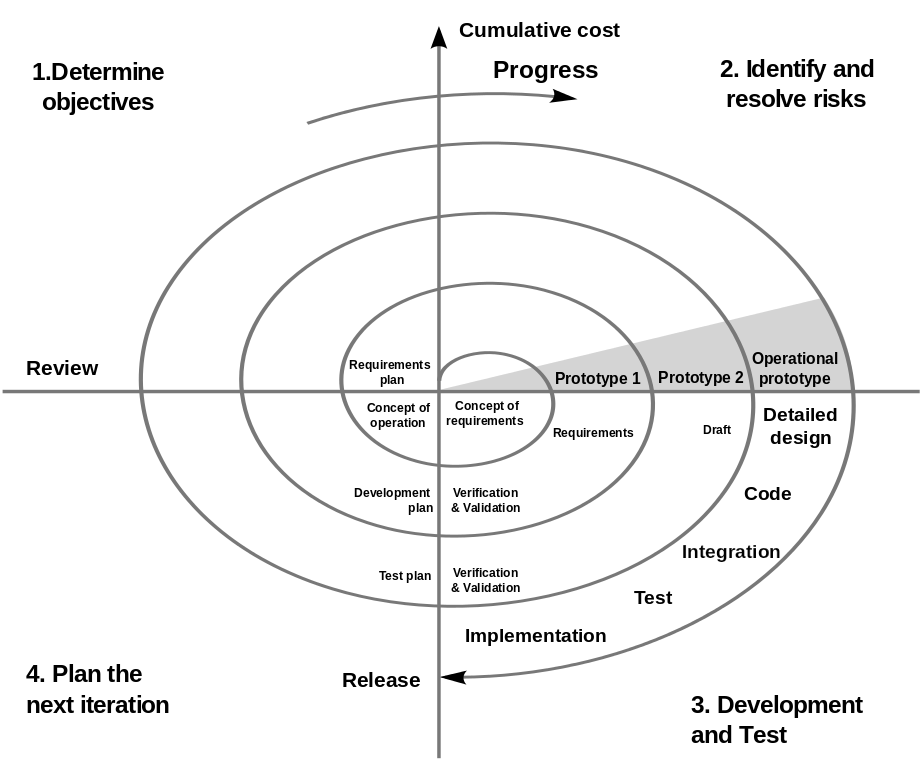
\includegraphics[width=0.45\textwidth]{figures/spiral-model.png}
\vskip 0.5cm}}
\caption{\protect\label{spiral-model} Spiral model }
\end{figure}

\vspace{.1in}

After the first round of risk analysis we discovered that this process is
detrimental to our development of the project and was over kill for our
needs. So we decided to change to the phased iterative and incremental
development model (IID). The IID model has the same basic features we wanted
from a process model of iteration based development with customer feedback
playing an important role. An illustration of how the IID model is used is shown
in figure \ref{iid-model}.

\vspace{.1in}

\begin{figure}[htb]
\fbox{\parbox[b]{.99\linewidth}{
\vskip 0.5cm
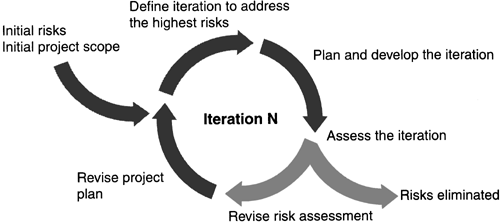
\includegraphics[width=0.45\textwidth]{figures/iid-model.png}
\vskip 0.5cm}}
\caption{\protect\label{iid-model} Incremental and Iterative development model }
\end{figure}

\vspace{.1in}

Settling on the IID model our team used it to some effect.
We planned to use each iteration to build up and refine features that were
developed in the previous iteration. To achieve this we started the first
iteration by creating a rough skeleton of a majority of the application with key
data models and function paths outlined.
After completing each iteration we had a meeting with our clients show casing the
new features that were added in the iteration cycle. With this meeting we also
took the opportunity to refine our knowledge of the requirements and receive
feedback on the work that we have completed.
Each iteration started with a rough plan of what is to be completed in that
iteration which in theory would of been refined as we gained more understanding
of the components.

%The experiences you made with using the process model and the lessons
% you learned from the project
\section{Experience}
% andrew: pretty kewl
% cuan: late?
% Cameron price (bread):
% Cameron Porter (no-bread):
% me: ~.~

The overall experience of using iterative and incremental development model was
good but had many places were we could improve next time. Through the
execution of the project we achieved our primary goal of using the model to get
the customer's feedback. This was one of the main reasons we chose the IID
process however we only had the opportunity to meet with the client two times.
Though the two client meetings resulted in a better understanding of the
requirements and expectations of the clients, only having two meetings
could not possibly result in a or near complete understanding of the
requirements for us to implement or even to give the clients enough of an idea of
what we have implemented so they can point out if we are going down the wrong
tack.
From this we only reached our third iteration cycle by the end of the project.
A critical error we made was to not have a clear plan to each iteration or even
have a deadline for the iteration to be completed by. With these missing aspects
of our iterations they were aimless and had no sense of urgency. This lead to
many team members to put this project on the back burner and left it till the
exam period. This resulted in iterations taking a long time to complete their
vague goals.

\vspace{.1in}

From the project I have learnt some important components to a successful group
project. In this project we agreed to try something that was new to most of the
team, using Ruby on Rails as our framework to build our application. We had one
member that was a professional in the framework and I was being tutored in the
framework in another group project. The other team members took this as a
learning opportunity to get to understand and use ruby and the Rails framework.
We also decided on using the Ruby on Rails framework for its strong use of the
model-view-controller (MVC) design pattern, see figure \ref{mvc-pattern}, that
separates the application into three distinct parts: logic, data, and display.
From these parts we divided out work with giving more back end focused work to
those more experienced with Ruby on Rails.

\vspace{.1in}

\begin{figure}[htb]
\fbox{\parbox[b]{.99\linewidth}{
\vskip 0.5cm
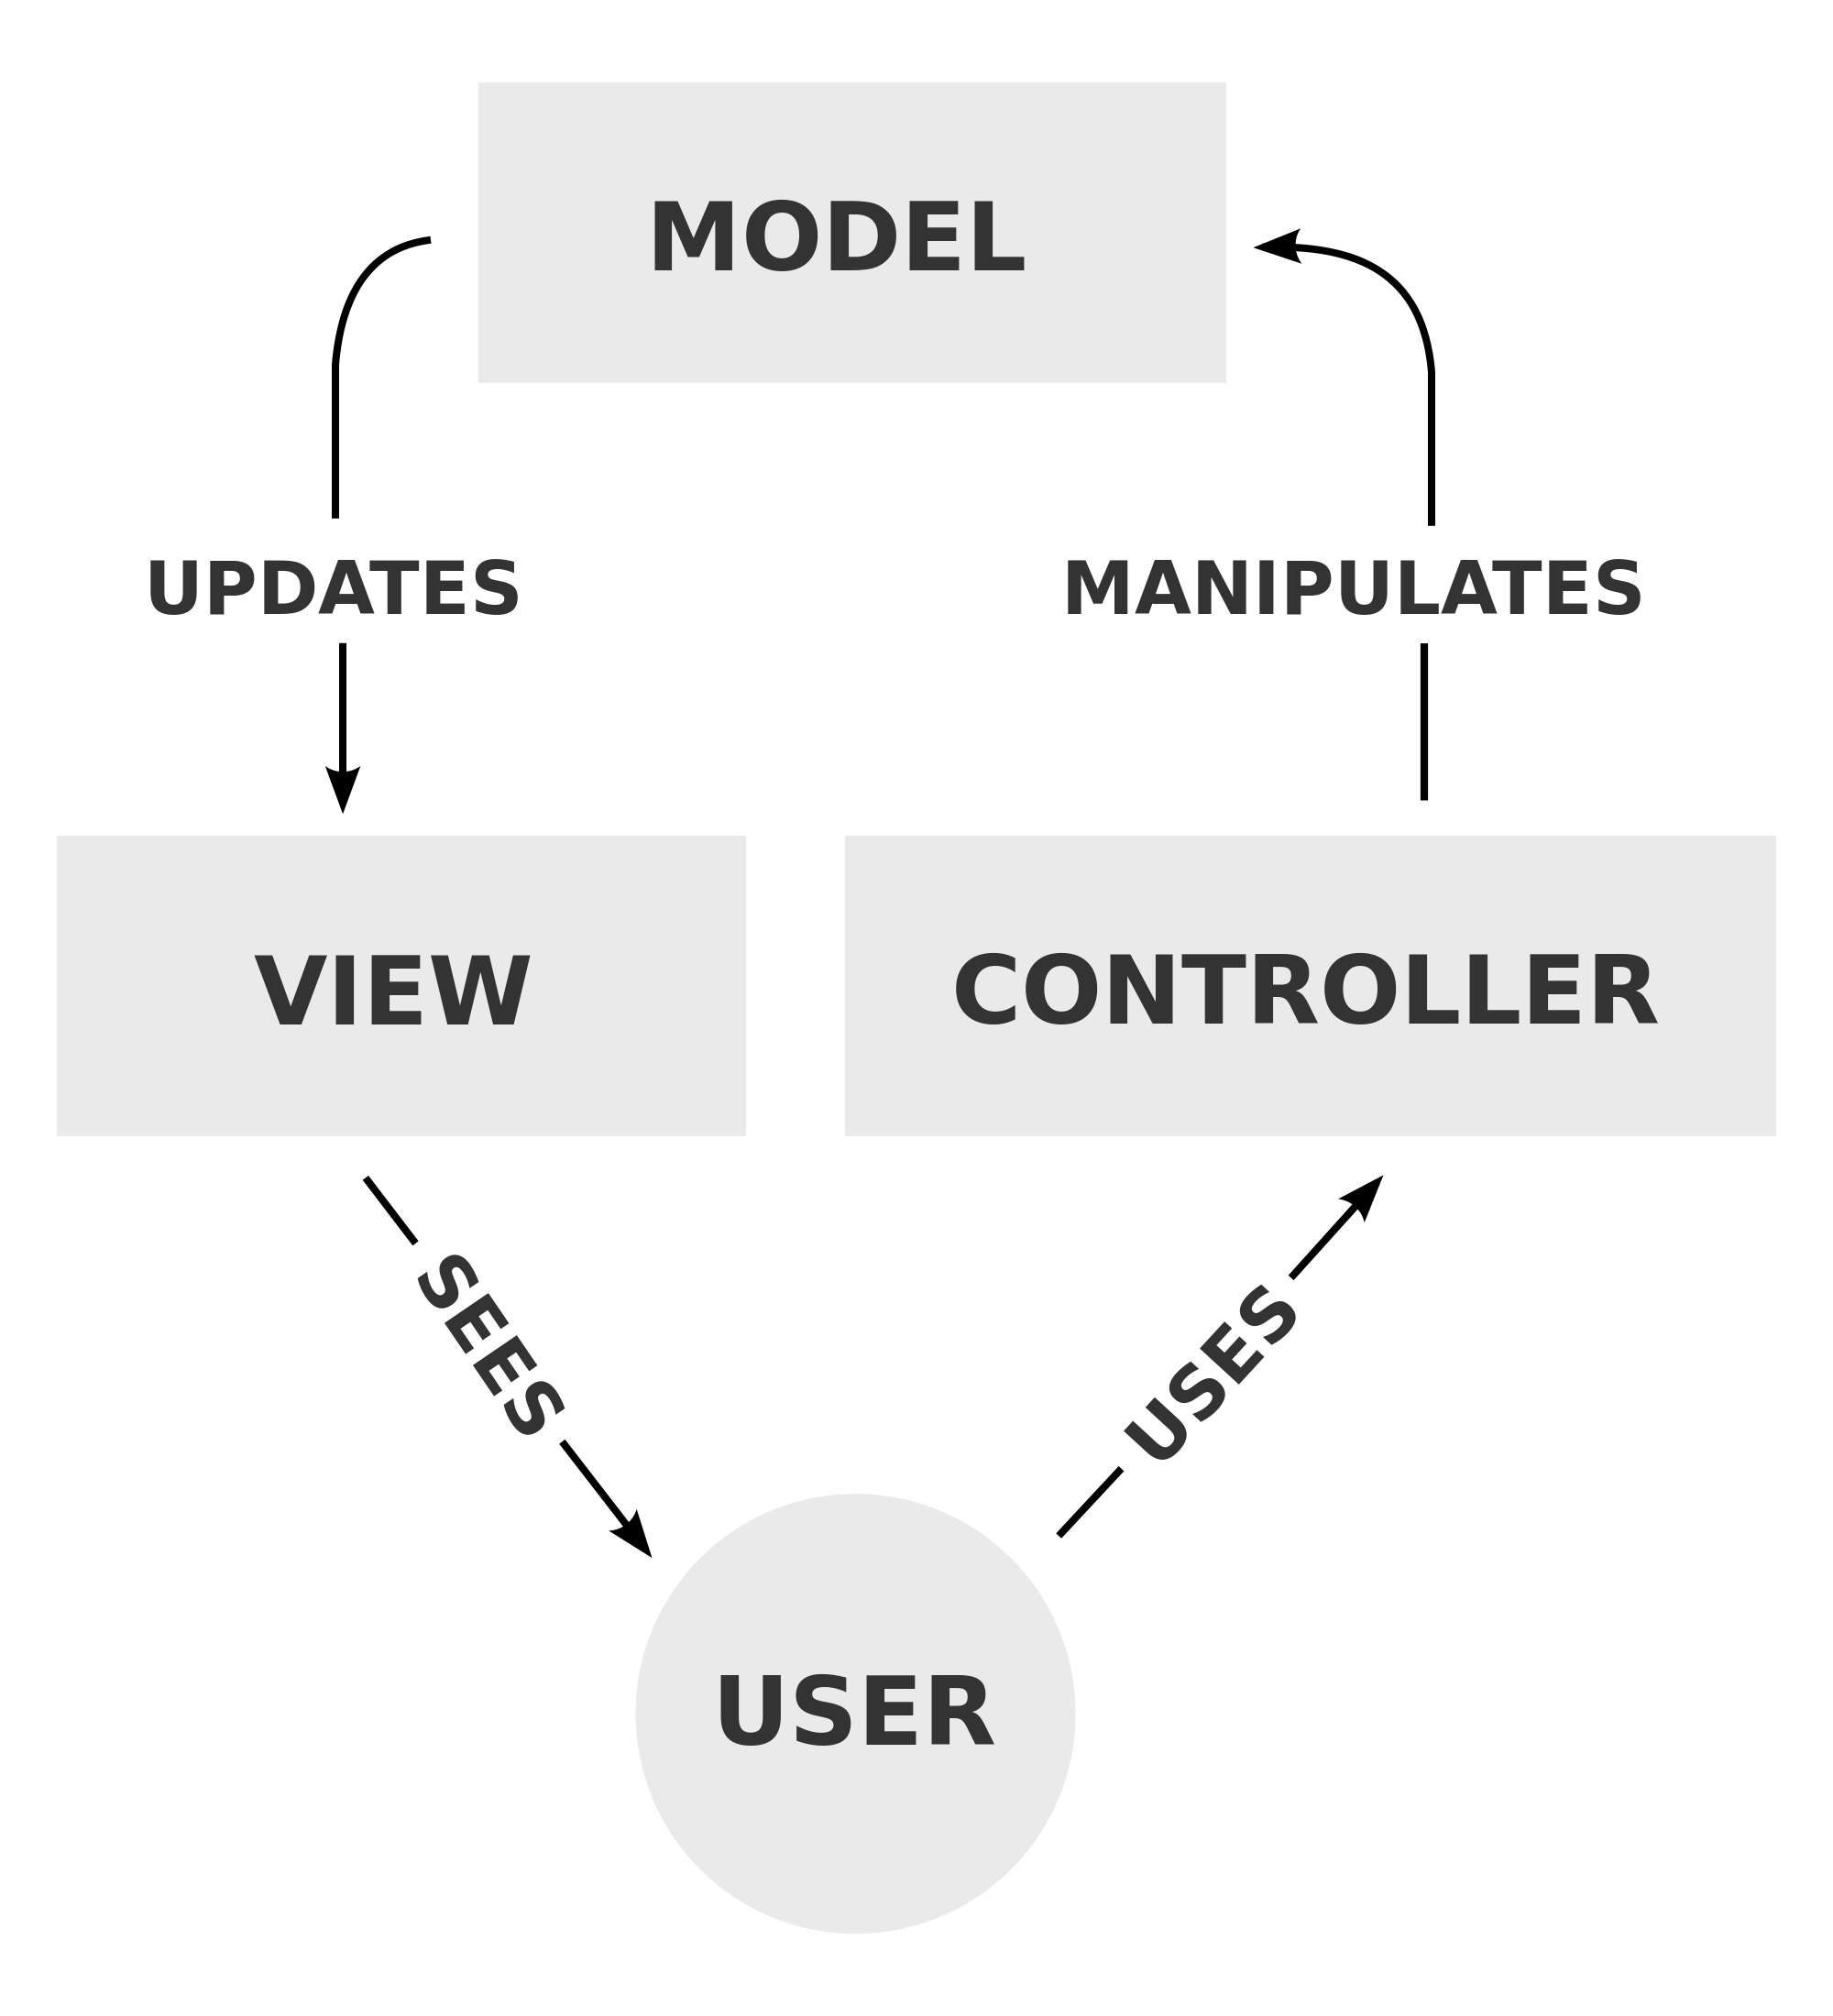
\includegraphics[width=0.45\textwidth]{figures/mvc.png}
\vskip 0.5cm}}
\caption{\protect\label{mvc-pattern} Model View Controller design pattern }
\end{figure}

\vspace{.1in}

For the first iteration I was apart of the sub-team to build the skeleton of the
application and wrote the baseline tests as a guide of how testing will be
carried out, as I was given the role of chief tester. From this the team agreed
to follow the feature branch and pull-request etiquette of using git and only
merge when the automated test suite passed. This allowed for a experimenting in the
branches while keeping the master branch clean of broken code.
Over the course of the project this method of using our tools worked well and
given another project with testing as a goal I would opt to use this
methodology of using git and automated testing again.

\vspace{.1in}

One the important components to a successful group project would be communication within the team.
Throughout the project our team communicated through online tools, such as
Slack, to organise team meetings and discuss portions of the work. The team
meetings were agreed to be a weekly meeting before a lecture with the goal of
talking about what is currently being done in the project and if you need help
speak up then. However these meetings were often derailed by unrelated talk or
looking back retrospectively some members that were struggling with foreign
frameworks and languages.
A side affect of the derailed meetings was the current goal of the project was
being poorly met, for example during the requirements gather phase most of the
talk was about which technologies should we use and attempting to solve the
problem before knowing what it was.
In the extreme this lead to one member ending up
contributing no code to the final product from what I gather was due to a
knowledge gap. In retrospect relying on people to speak up about not understanding
something is not the best method to resolve a knowledge gap but should be more
insistent and direct with asking members about their progress.
From this I have learnt that a meeting is only effective when it is on task and
the goals of the meeting is met. For my next project I would attempt to be
stricter in meeting to keep it on task instead of allowing members to get off topic
and start talking about their world trip they are planning otherwise it just
turns into a waste of time.

\vspace{.1in}

Time management is also a key component to a successful group project.
During the project we had weekly meetings to keep everyone everyone update to
date on the project. However the turn out for the meetings were not prefect,
especially when additional working meetings were held. This was
due to the differing schedules and courses between the members. While other
courses were becoming more time consuming we discussed wither or not keep our
same meeting. In the end we chose to keep the same meeting time, though it did
end up with keeping a similar scenario. Looking back at this there was two
options to ensure attendance. One option would to change the time to a more
fitting time to compensate for the other courses, or be more strict about
attendance and excuses for tardiness. However I do not think either of these
options would of resulted in overall positive outcome for the project as a
whole. Another aspect of time management that is important is to place dead
lines on work. For instance we should of put deadlines on our iterations or at
least the individual portions of work that lossy made up an iteration. As a
result of this we kept pushing back client meetings so we could get the features
that we thought that were suppose to be in the iteration. If I were to run
another project in an IID method again this, and setting a clear goal for the
iteration, would be the most important part of this model I have learnt from
being apart of this project.

% How well your application meets the requirements gathered during the
% initial requirements analysis and what you have done to ensure your
% application meets the requirements
\section{Requirements}
% not all features
% ensure meeting requirements with testing and checking against our use cases

The KPSmart clients provided us with an outline of the requirements of the
system and further went into detail during client meetings or while the clients
were available.


% What kind of system is your application, i.e., S-system, E-system or P-
% system and why?
\section{System Type}
% Define, what the 3 system types are
% point out which parts of the system display symptoms of that system
% and which points it misses
% big reveal it is P-System!!!

A software program can be described as one of three types of systems:
S-System, E-System and P-System. Each type of system has a varying set of traits
to their development and maintenance cycles as they have different relationships
to their environments and specifications that they were designed for and how
they react to changes in either of them. These range from development
and maintenance is continuous to after development there is no need for
maintenance. The KPSmart application displays some traits of each of system
types but mostly exhibits the traits of a P-System.

\subsection{S-System}

The KPSmart application has some traits of a S-System. Which are broadly described as
systems which has its functionality formally defined by the specification as
well as how it will be delivered \cite{lehman:1980}.
This focus on specification is what puts the \emph{S} into \emph{S}-System.
In practice S-Systems are systems which solve a problem which is related to the real world
with very rigid rules such as implementing a sorting algorithm which leads onto a set of well defined
specifications for the system to be implemented.
Changing the specifications, and thus the problem the system is to solve,
would results in changing the system as a whole due to the system being tightly
coupled. The maintenance of a S-System would be low as the resulting system
would not need to change unless its specifications does.
This process is illustrated by the figure \ref{s-system}.

\vspace{.1in}

\begin{figure}[htb]
\fbox{\parbox[b]{.99\linewidth}{
\vskip 0.5cm
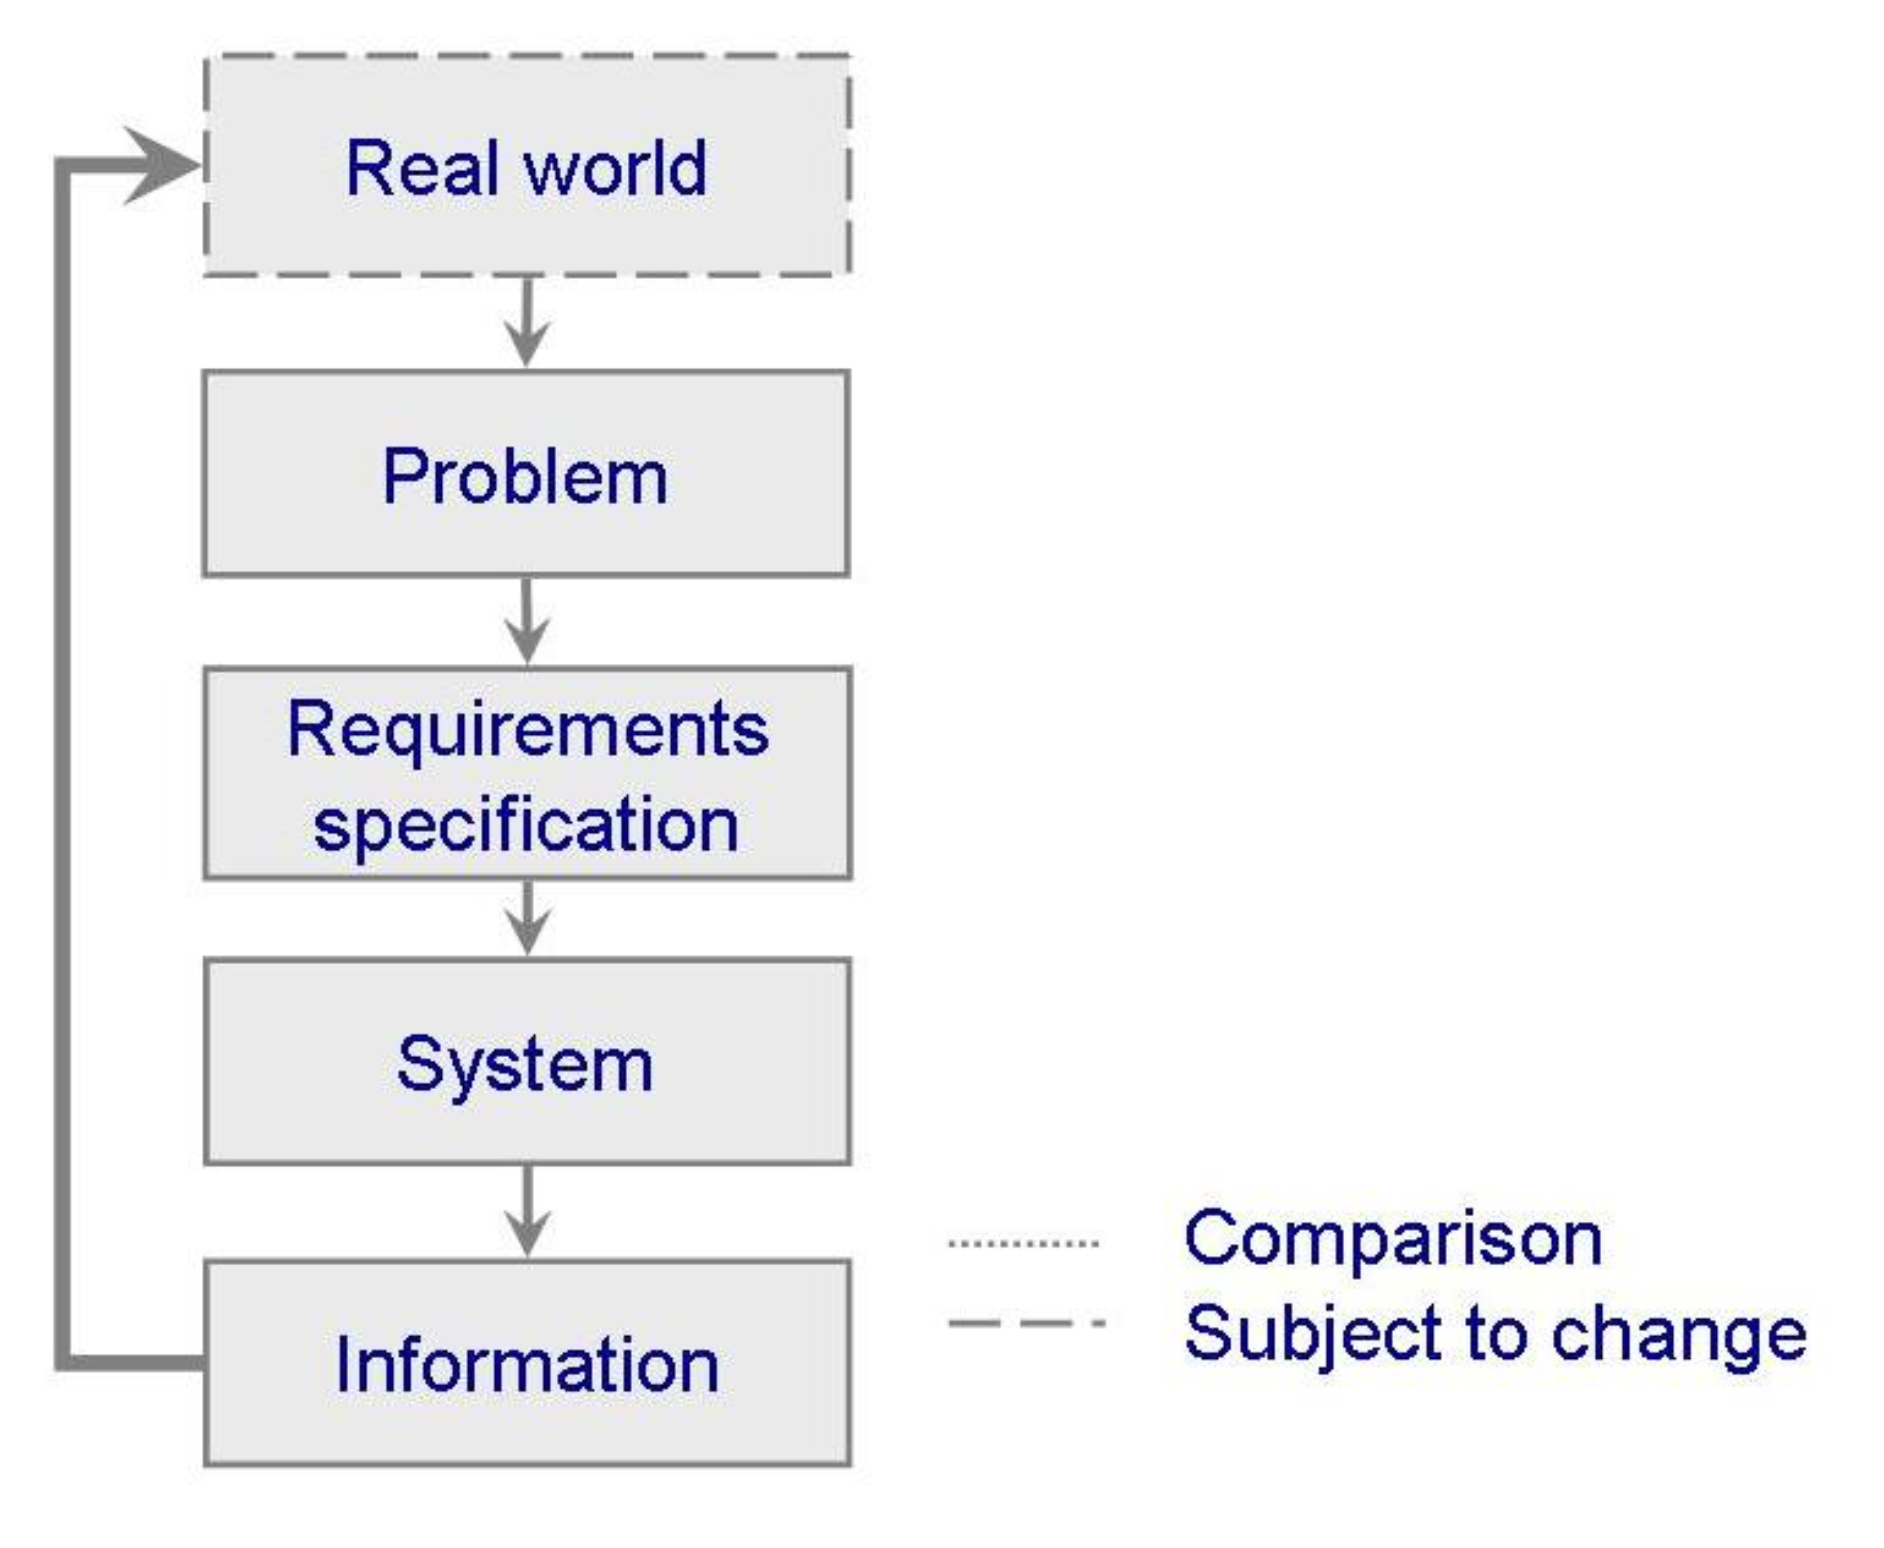
\includegraphics[width=0.45\textwidth]{figures/s-system.png}
\vskip 0.5cm}}
\caption{\protect\label{s-system} S-System}
\end{figure}

\vspace{.1in}

The KPSmart application itself is formally defined by specifications to solve a
problem but lacks the level of details and rigidity to classify it as an
S-System, however some sub-systems of the applications are fit to be classed as such.
These include the routing and the calculation for a mail delivery duration
sub-systems as they both are well defined in what problem they solve.
However the KPSmart application as a whole is not a S-System.

\subsection{E-System}

The KPSmart application has some aspects of an E-System.
An E-System is a type of system which is embedded in apart of the problem and is
apart of environment of the problem itself \cite{lehman:1980}. A practical example of this would be
a stock market trader AI, which itself is apart of the market and must not only
model the environment which it is trading in but also model its own impacts on the market
so it can maximise yields. The drive to model and interact with the environment
is the trait which gives this types of system the name of \emph{E}-System for
an environment system. With this kind of system the specifications and models
of the system are all derived from a problem residing the real world which
informs the views and models to create abstractions over the problem. From these
abstractions a set of requirements and specifications are drawn up to create a
system that will exist in the same world as the problem. However the resulting
system will likely cause changes to the problem and world around it leading to
a feedback loop of changes in models and requirements into how the system
changes the world. The system would need to also model itself and it changes to
the world around it to be effective in situations twitch stock trading or
dispatching airplanes. This process is illustrated by the figure \ref{e-system}.

\vspace{.1in}

\begin{figure}[htb]
\fbox{\parbox[b]{.99\linewidth}{
\vskip 0.5cm
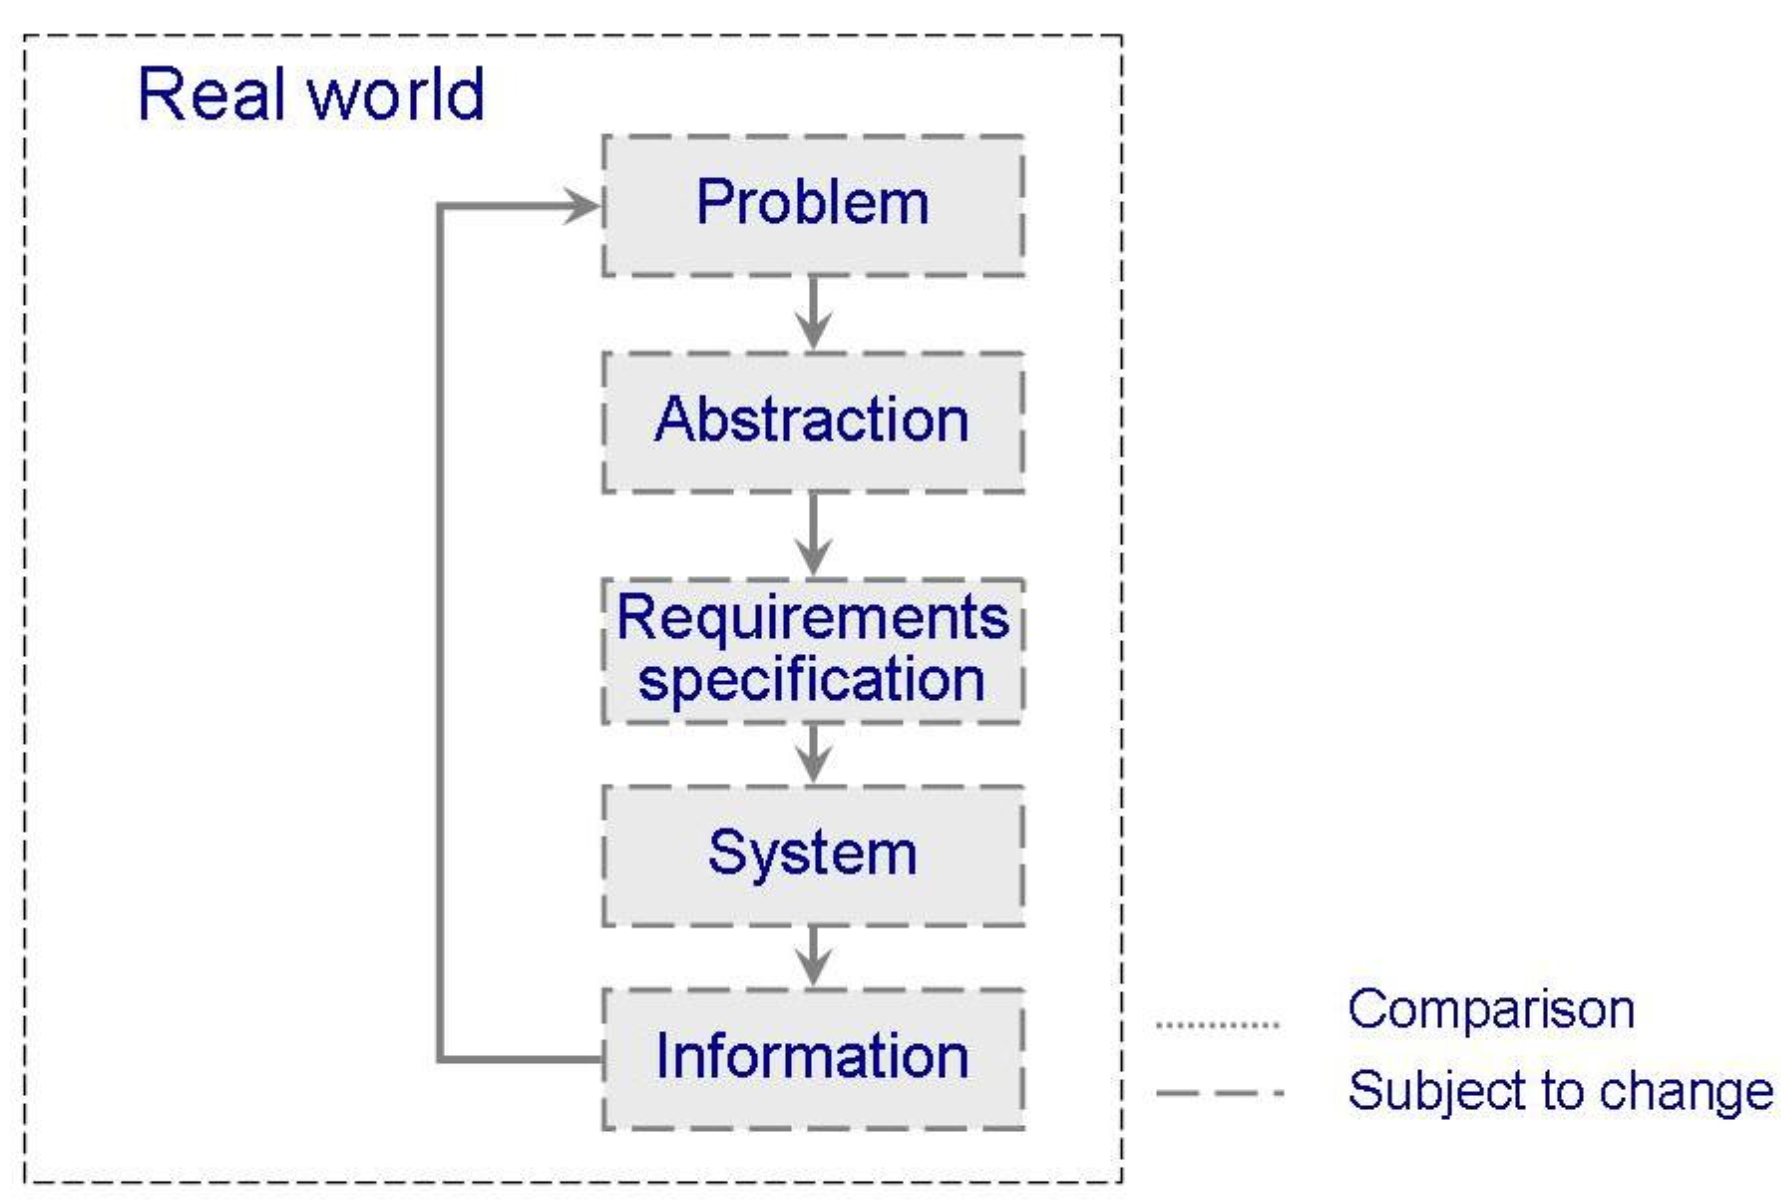
\includegraphics[width=0.45\textwidth]{figures/e-system.png}
\vskip 0.5cm}}
\caption{\protect\label{e-system}  E-System }
\end{figure}

The KPSmart application has some sub-systems and features which could
be consider to be E-System-like. These elements are most prevalent in
the manager tooling. For example the decision support functions of suggesting
to close or open routes to maximise profit as well as suggesting that a route
price is too high and could improve volume with a reduction. These types of
features would benefit from modeling the real world with the KPSmart application
as an actor in it. However the KPSmart application as a whole is not a E-System.

\vspace{.1in}

\subsection{P-System}

The KPSmart application has many, if not all, of the traits of a
P-System. A P-System is the middle ground between an E-System and a
S-System, it has a clear set of specifications for the system to
implement as a base of the problem as well as more functionality that
builds upon the base to create more complex \cite{lehman:1980}. An
example of a P-System would be a computer controlled player for a game,
such as checkers, while the base game is well defined and specified it
will also need to make the best decision in its current situation.
The P-System is built using an abstraction of a problem from the world
at large, which is then used to define the requirements and specifications
of the system. The built system may reveal more information about the problem
that could require a rethink or an update to the abstraction of the problem,
thus leading onto changes in the specifications and the system. This can form
a feedback loop similar to an E-System but does not need to model the affects
that the system will have on the problem as it is detached from it.
The maintenance of a P-System would be more revolving around new information
arising about the problem to improve the abstractions and requirements that for
the system on top of the general maintenance work.
This process is illustrated in figure \ref{p-system}.

\vspace{.1in}

\begin{figure}[htb]
\fbox{\parbox[b]{.99\linewidth}{
\vskip 0.5cm
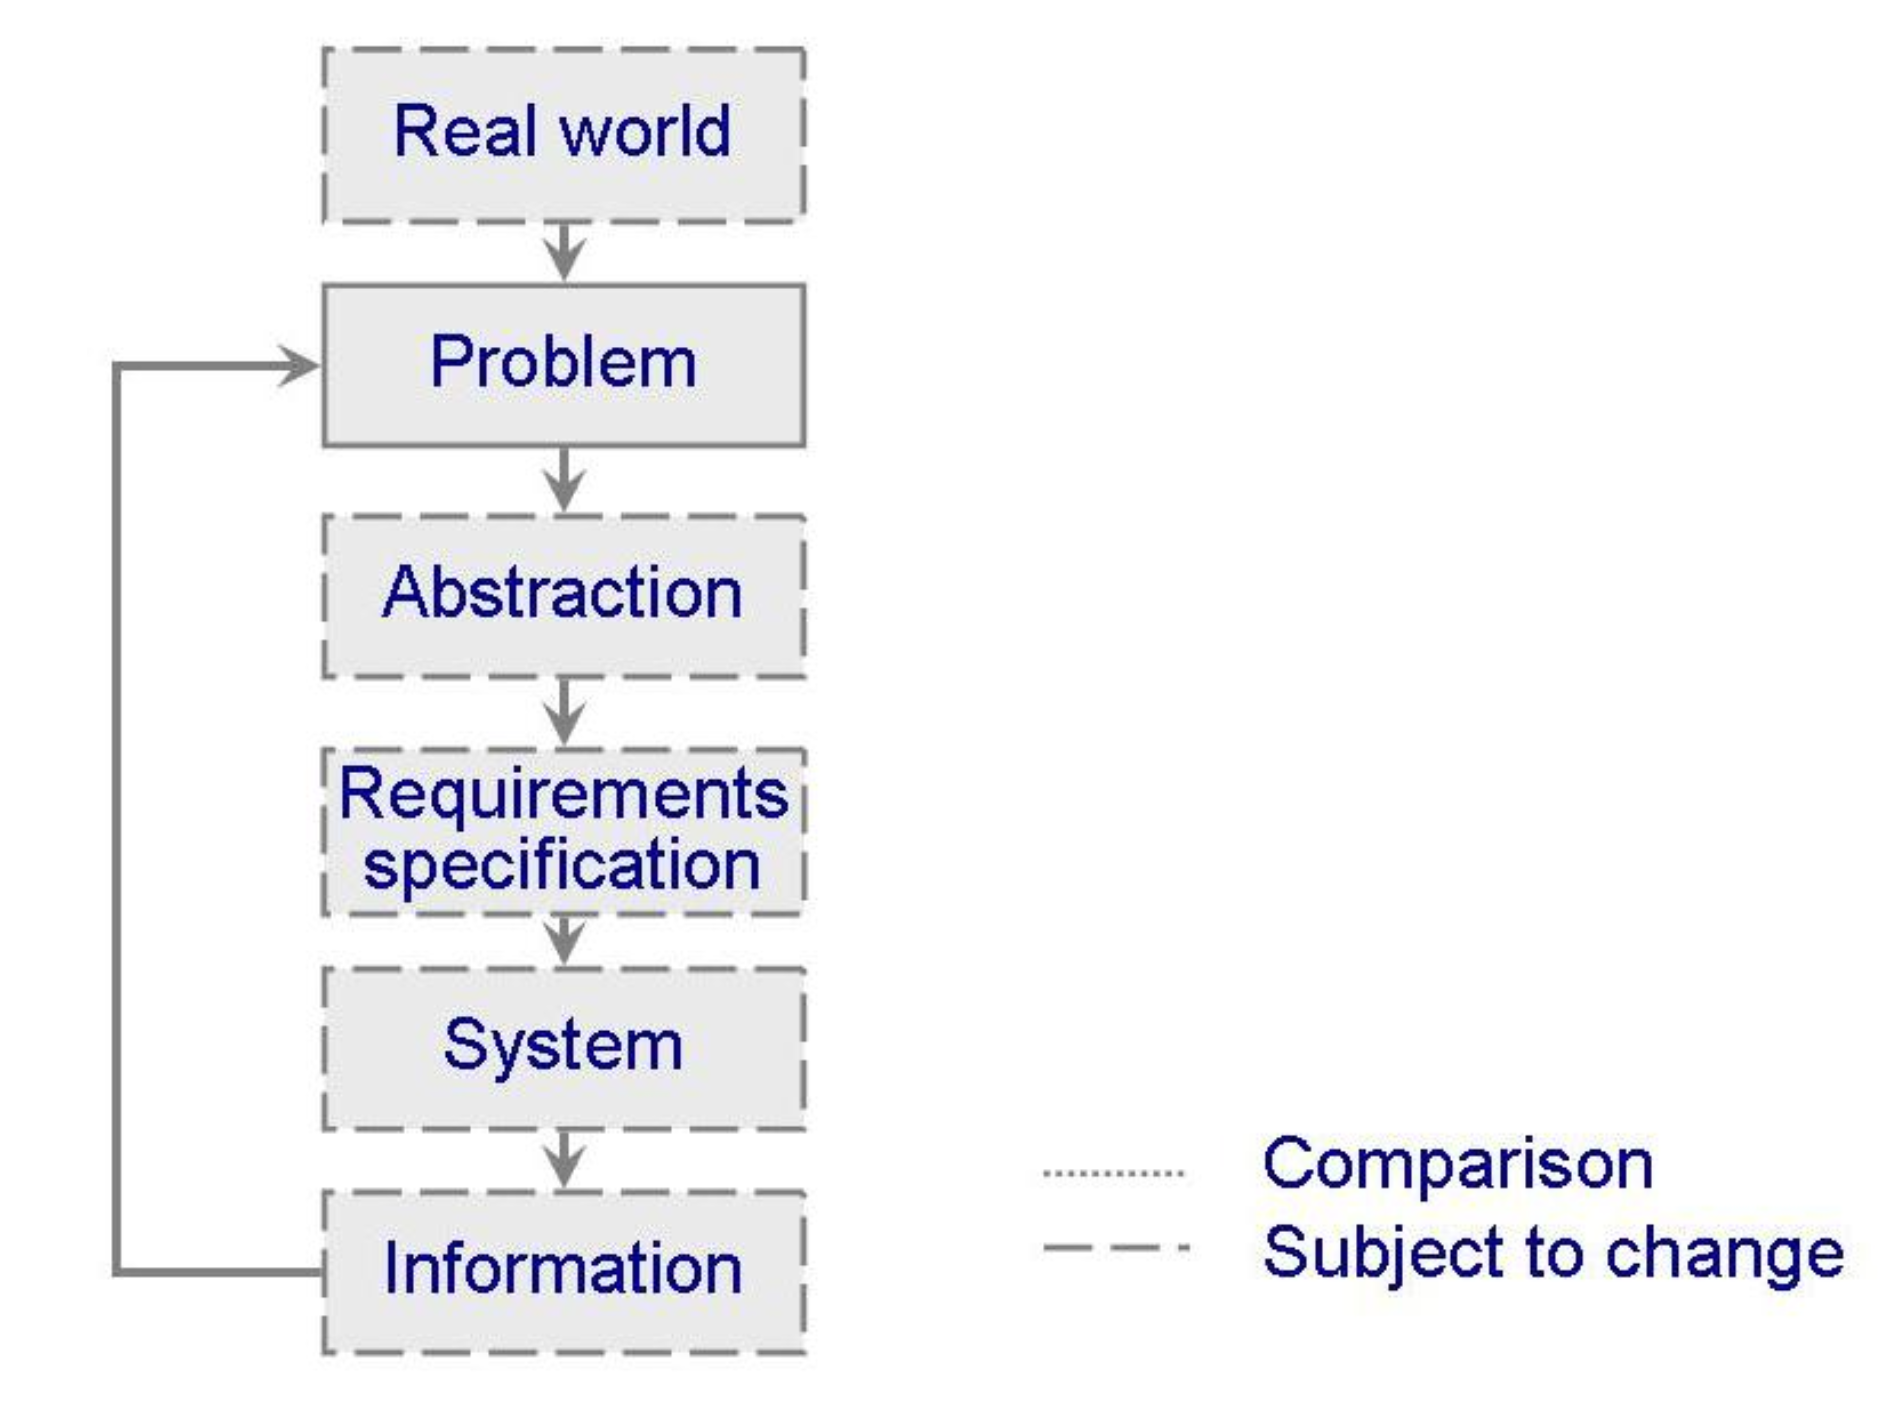
\includegraphics[width=0.45\textwidth]{figures/p-system.png}
\vskip 0.5cm}}
\caption{\protect\label{p-system}  P-System }
\end{figure}

\vspace{.1in}

The KPSmart application is a P-System. This is because of its initial set of
requirements describing the problem the system are not holistic enough to
implement it as an S-System nor is it embedded in and changing the world of mail
delivery logistics thus not an E-System. In addition to these a lack of
these features the system is an abstraction of the business process that the
KPS firm wanted to automate and their requirements and specifications grew over
time with greater understanding of the problem so did the system. With these
traits and the system on the whole is a P-System even though some sub-systems
could be defined as S-Systems or E-Systems.

% What kind of maintenance activities may be needed to maintain the
% application. Recall that four types of software maintenance activities were
% discussed in the lectures.
\section{Maintenance}
% Corrective (control over day-to-day):
%
% Adaptive (control modifications):
%
% Perfective (perfecting existing funcs):
%
% Preventive (prevent performance degrade):
%   Database queries for reports are slower than they should be

The developed KPSmart application however grand or functional it is will need
to be maintained, and most likely not by its original authors. This maintenance
could take one of four different forms: corrective; adaptive; perfective, and;
preventive. The KPSmart applications as it stands would benefit from each of
these maintenance activities and some work has already be done from the original
developers to help lessen the pain of these activities.

\cite{Pigoski:1996}

% What process model would you use if the project were developed as an
% open source application, and why?  Which Indirect Sale-Value model,
% discussed in the lecture, can be used for your application, and how?
\section{Open source}

\cite{raymond:1999}

\section{Conclusion}

\bibliographystyle{agsm}
\bibliography{report}

\end{document}

% vim:set spell et sw=4 ts=4 tw=80:
